\documentclass[11pt]{article} % use larger type; default would be 10pt

\usepackage[utf8]{inputenc} % set input encoding (not needed with XeLaTeX)
\usepackage[ngerman]{babel}% deutsche Trennregeln
\usepackage[T1]{fontenc}% wichtig für Trennung von Wörtern mit Umlauten

%%% PAGE DIMENSIONS
\usepackage{geometry} % to change the page dimensions
\geometry{a4paper, left=30mm, right=40mm, top=25mm, bottom=20mm} 

%%%%%%%%%%%%%%%%%%
% Mathe Packages %
%%%%%%%%%%%%%%%%%%

\usepackage{amsmath}
\usepackage{amsthm}
\usepackage{amssymb}





%%%%%%%%%%%%%%%%%%%%%%%%%
% Mathematische Symbole %
%%%%%%%%%%%%%%%%%%%%%%%%%

\newcommand{\N}{\mathbb{N}}
\newcommand{\Z}{\mathbb{Z}}
\newcommand{\R}{\mathbb{R}}
\newcommand{\C}{\mathbb{C}}
\newcommand{\Q}{\mathbb{Q}}
\newcommand{\A}{\mathbb{A}}
\newcommand{\Aq}{\A_\Q}
\newcommand{\kinf}{k_\infty}
\newcommand{\ginf}{g_\infty}
\newcommand{\tinf}{t_\infty}
\newcommand{\finf}{f_\infty}
\newcommand{\xinf}{x_\infty}
\newcommand{\xiinf}{\xi_\infty}
\newcommand{\finft}{\hat{f}_\infty}


%%%%%%%%%%%%
% Theoreme %
%%%%%%%%%%%%



\theoremstyle{definition}
\newtheorem{defi}{Definition}[section]
\newtheorem{bsp}[defi]{Beispiel}

\theoremstyle{plain}
\newtheorem{satz}[defi]{Satz}
\newtheorem{lemma}[defi]{Lemma}



\begin{document}

\pagenumbering{Roman}

%%%Deckblatt


%%% Inhaltsverzeichnis
\tableofcontents
\clearpage

\pagenumbering{arabic}   



%%%%%%%%%%%%%%%%%%%Beginn

\section{Einleitung}
\label{sec:kapitel1}

\clearpage

\section{Die Hausarbeit in der Praxis}
\label{sec:kapitel2}




Hier steht ein kurzer einleitender Text zwischen den beiden Überschriften.



\subsection{Die Quellenverwaltung und Zitiertechnik}
Für die Quellenverwaltung empfehlen wir die Software Citavi, welche unter folgendem Link kostenlos zu beziehen ist: \underline{http://citavi.com/de/download.html}\\
Als Zitationsstil ist der Citavi Basis-Stil (deutsch) zu werden, was den Grundeinstellungen entspricht (bzw. Citavi Default Style (englisch)).
\begin{figure}[!htb]
\centering
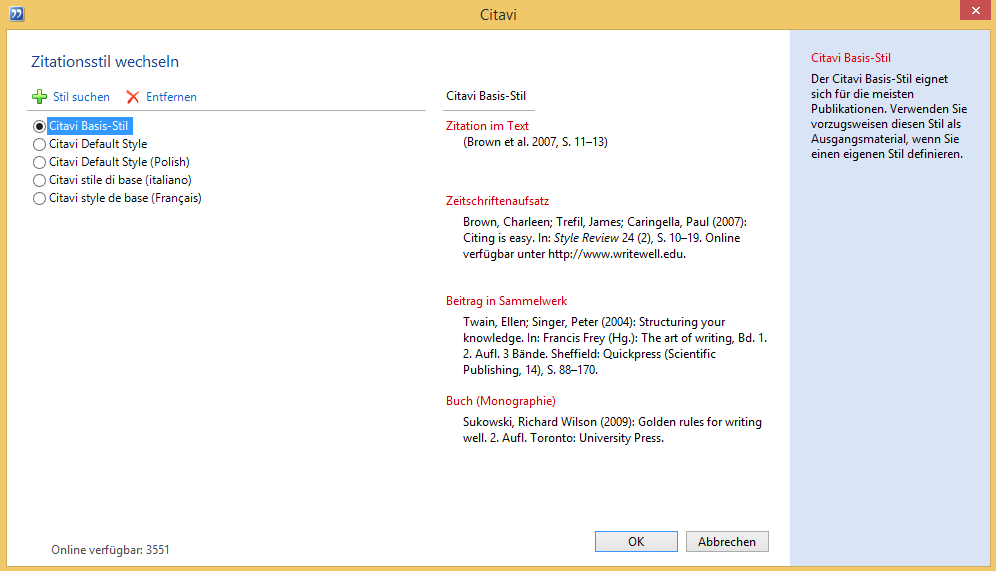
\includegraphics[scale=0.45]{Bilder/Citavi.png}
\end{figure}

Zitate sind grundsätzlich in den Fließtext einzufügen. Fußnoten werden für Zitate nicht genutzt. Nur wenn eine Einbindung der Information in den Text nicht möglich oder sinnvoll ist, kann eine Fußnote genutzt werden. Direkte Zitate sollten vermieden, stattdessen indirekte Zitate bevorzugt werden. Inhalte von Fußnoten sollten möglichst in den Text eingearbeitet werden.
$\;$\\
\begin{spacing}{1}
\textbf{Beitrag in einem Sammelband}\\

Beispiel Literaturangabe:\\

Degele, Nina (2005): Neue Kompetenzen im Internet. In: Kai Lehmann und Michael Schetsche (Hg.): Die Google-Gesellschaft. Wissen im 21. Jahrhundert. Bielefeld: transcript, S. 63–74. \\

\textbf{Buch (Monographie)}\\

Beispiel Literaturangabe:\\

Andretta, Susie; Dervall, John; Li, Han (2005): Information literacy. A practitioner's guide. Oxford: Chandos (Chandos information professionals series). \\

\textbf{Hochschulschrift}\\

Beispiel Literaturangabe:\\

Zweifel, Aron (2005): Information Literacy Konzeption eines Teaching Library-Moduls am Beispiel der Fachhochschulbibliothek Frankfurt am Main. Diplomarbeit. Fachhochschule Frankfurt a. M., Frankfurt a.M. Online verfügbar unter\\ www.fh-frankfurt.de/de/.media/bibliothek/aronzweifel-ilkonzeption-tlmoduls-fh-ffm.pdf, zuletzt geprüft am 30.01.2009.\\

\textbf{Internetdokument}\\

Beispiel Literaturangabe:\\

Arbeitsgemeinschaft Informationskompetenz NRW (2005): ULB Bonn - AG Informationskompetenz - Schulungs- und Lernmaterialien. Online verfügbar unter\\ www.informationskompetenz.de, zuletzt aktualisiert am 24.04.2005, zuletzt geprüft am\\ 30.01.2009.\\
\end{spacing}

Internetzitate werden analog zu den direkten und indirekten Zitaten genutzt. Eine Internetquelle ist nur dann zu zitieren, wenn ein Autor und ein Erscheinungsjahr für die Quelle verfügbar sind.\\

\begin{spacing}{1}

\textbf{Zeitschriftenaufsatz}\\

Beispiel Literaturangabe:\\

Correia, Ana Maria Ramalho; Teixeira, José Carlos (2003): Information literacy. An integrated concept for a safer Internet. In: Online Information Review 27 (5), S. 311–320.\\

\textbf{Zitation im Text:}\\

Beispiele:\\

Ein Autor: (Degele 2005, S. 63)\\
Zwei Autoren: (Correia und Teixeira 2003, S. 319)\\
Ab drei Autoren: (Andretta et al. 2005, S. 5)\\

\end{spacing}

Jedes Werk, aus dem zitiert wurde, muss im Literaturverzeichnis aufgeführt werden. Werke, die zur Erarbeitung des Themas genutzt aber nicht zitiert wurden, gehören nicht ins Literaturverzeichnis. \\

Die Universitätsbibliothek bietet Ihnen mit dem Literaturverwaltungsprogramm RefWorks ebenso ein persönliches und kostenfreies Tool für die professionelle Verwaltung Ihrer Literaturangaben. Weitere Informationen finden sich auf der Uni-Homepage:\\http://www.bibliothek.uni-augsburg.de/service/literaturverwaltung/refworks/









\clearpage


\subsection{Der Schreib- und Forschungsprozess}

\begin{figure}[h]
\centering
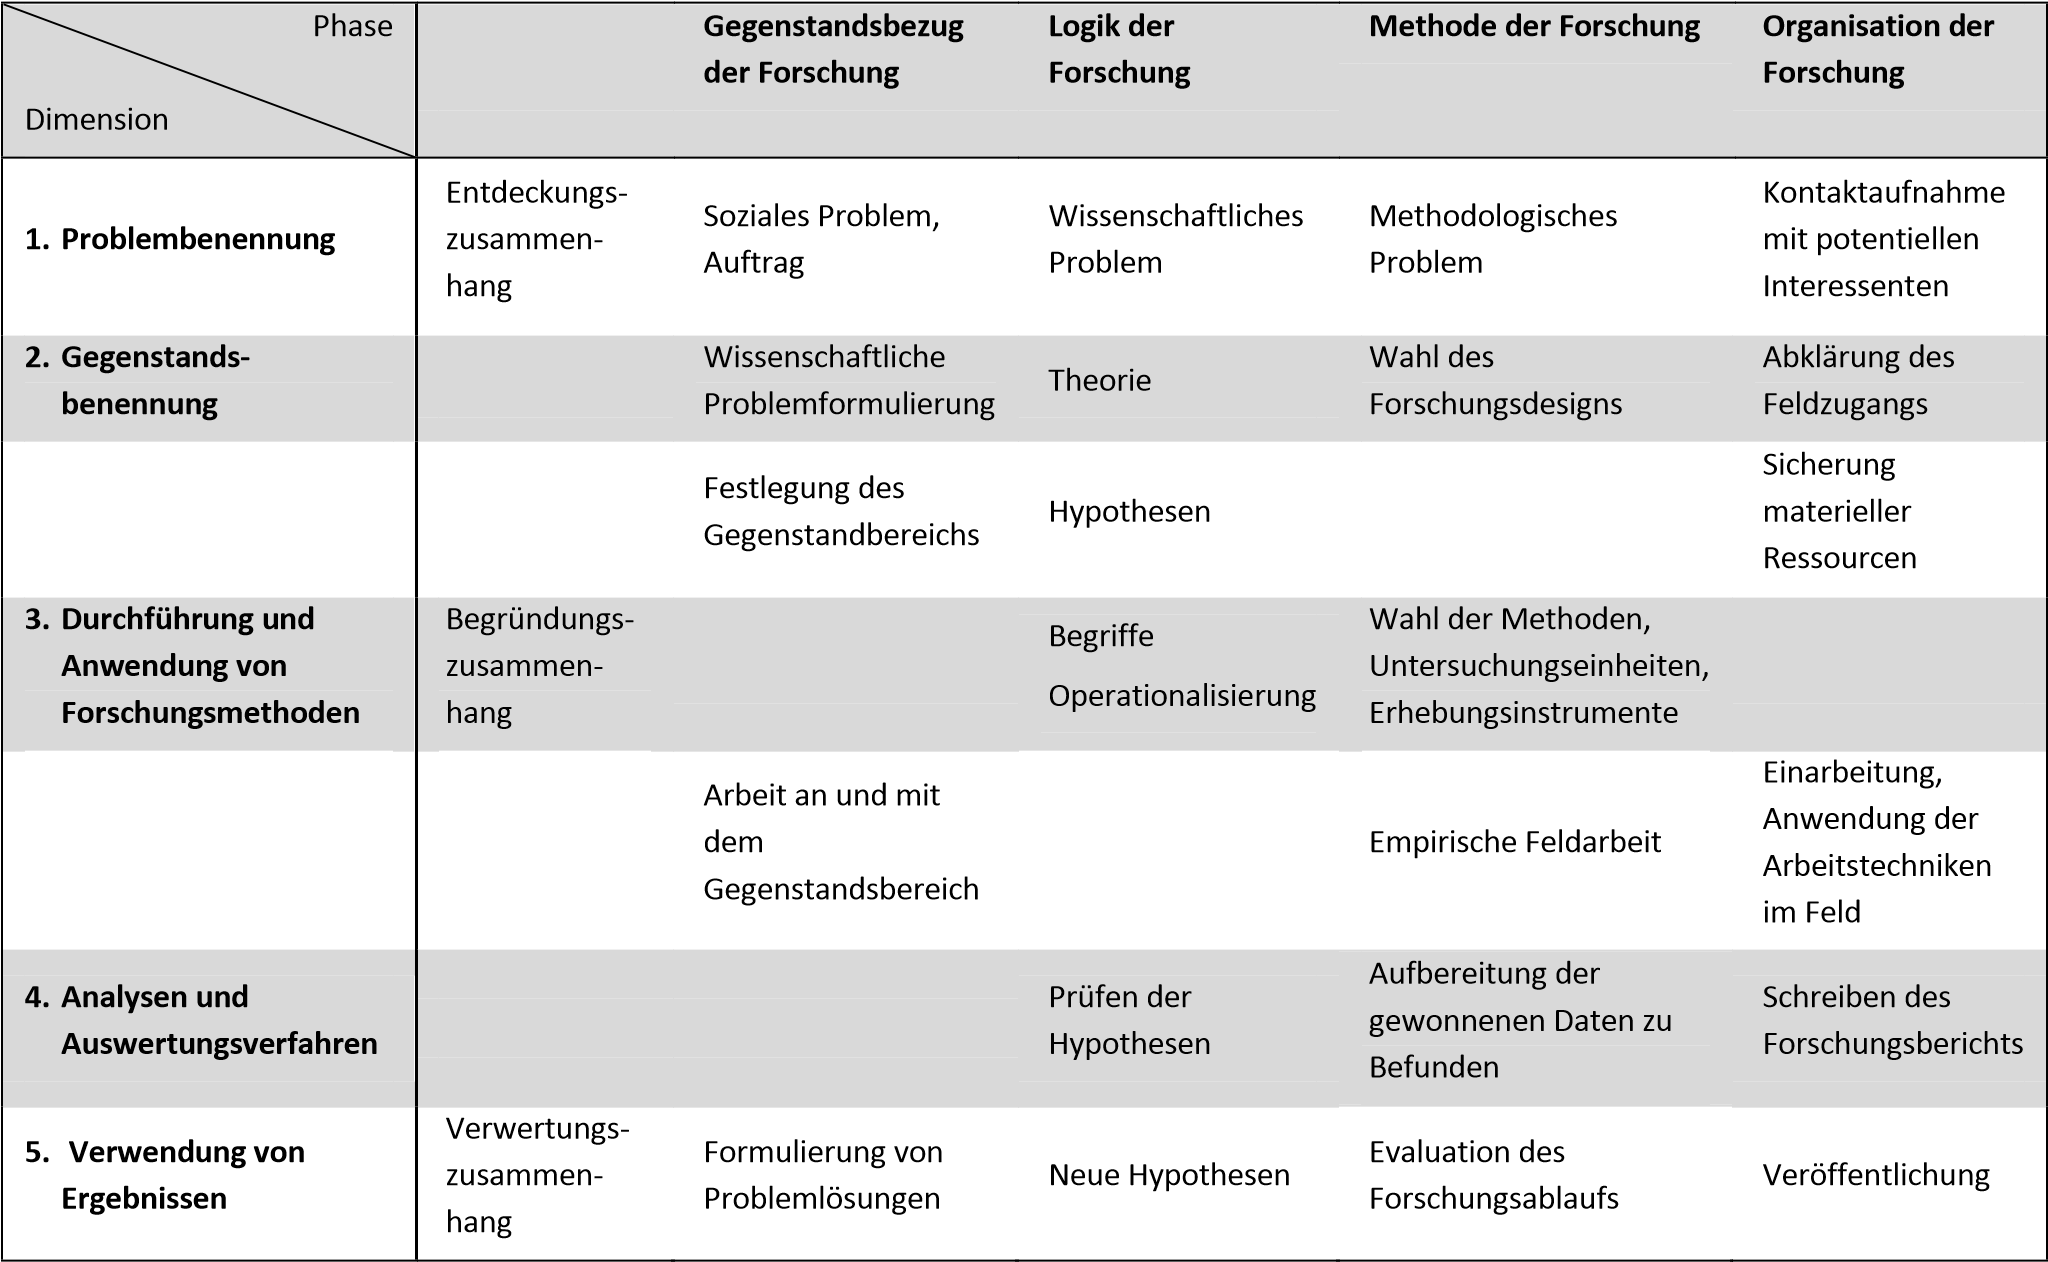
\includegraphics[width=1\textwidth]{Bilder/Abbildung.png}
Quelle: \citet{atteslander2010}, S. 13
\caption{Dimension einer wissenschaftlichen Arbeit nach Peter Atteslander}
\label{abb:abbildung1}
\end{figure}










\clearpage



\subsection{Bestandteile einer wissenschaftlichen Arbeit}


\begin{table}[htbp]
\renewcommand{\arraystretch}{1.4} 
  \centering

    \begin{tabular}{|l|l|}
\hline
    \textbf{{\large Hauptgruppe}} &  \textbf{{\large Bestandteile}} \\  \hline
    Titel &  $\cdot \quad$ Titelblatt \\ \hline
    Einleitungsapparat &  $\cdot \quad$ Abstract \\
	& $\cdot \quad$ Inhaltsverzeichnis \\
          &  $\cdot \quad$ Abbildungsverzeichnis \\
          &  $\cdot \quad$ Tabellenverzeichnis \\
	&  $\cdot \quad$ Abkürzungsverzeichnis \\ \hline
    Einführung &  $\cdot \quad$ Kurze Hinführung zum Thema \\ \hline
    Hauptteil &  $\cdot \quad$ Detaillierte Behandlung des Themas  \\ \hline
    Schluss &  $\cdot \quad$ Zusammenfassung und Ausblick \\ \hline
    Abschlussapparat & $\cdot \quad$ Anhang \\
	& $\cdot \quad$ Literaturverzeichnis \\
          &  $\cdot \quad$ Eidesstattliche Erklärung \\ \hline

    \end{tabular}%
  \label{tab:tabelle1}%



$\;$\\

\caption{Bestandteile einer wissenschaftlichen Hausarbeit}

Quelle: \citet{atteslander2010}, S. 13

\end{table}
Tabellen und Abbildungen unterstreichen Aussagen und illustrieren Forschungsergebnisse, um deren Verständnis für den Leser zu erleichtern. Sie dürfen nur dann eingesetzt werden, wenn sie im Text ausführlich erläutert werden. Bitte achten Sie darauf, dass die Tabellen selbsterklärend und notwendige Inhalte in die Tabellenbeschreibung aufzunehmen sind. Qualitativ müssen alle Abbildungen und Tabellen so hochwertig sein, dass sie sowohl auf dem Bildschirm, als auch auf einem Ausdruck klar und deutlich lesbar sind. Formal benötigt jede Abbildung eine Abbildungsunterschrift, jede Tabelle eine Tabellenüberschrift. Außerdem ist jeweils eine Quellenangabe, entsprechend der Zitation im Text, anzufügen.\\
Stilistisch ist auf eine neutrale Formulierung zu achten. Formulierungen mit „ich, man, wir, es“ sollten unbedingt vermieden werden.







\clearpage

\section{Riemanns Beweis}
\label{sec:kapitel3}

Wenden wir die Poisson-Summenformel f\" ur $\kinf$ auf die Schwartz-Funktion $\ginf(\xinf):=e^{-\pi|\xinf|^2}$ an, sehen wir, dass die Thetafunktion
\begin{align}
	\Theta_\infty (\xinf):=\sum_{n\in\Z}{\ginf (n\xinf)} = 1+ 2\sum_{n=1}^\infty{e^{-\pi n^2 |\xinf|_\infty^2}}
\end{align}
die Funktionalgleichung
\begin{align}
	\label{eq:thetafunktional}
	\Theta_\infty (\xinf) = \frac{1}{|\xinf|_\infty} \Theta_\infty(\frac{1}{\xinf})
\end{align}

f\"ur $\xinf \in \kinf^\times :=\kinf\setminus{0}$. Da insbesondere $\Theta_\infty(x_\infty)-1$ f\"ur $\xinf \rightarrow \infty$ schnell f\"allt, sehen wir, dass $\Theta_\infty(\xinf) - 1 / \xinf$ schnell f\"allt wenn $\xinf \rightarrow 0$. 
Formal k\"onnen wir die Mellin-Transformation auf \eqref{eq:thetafunktional} anwenden und folgern
\begin{align}
	\label{eq:thetamellin}
	\int_{k_\infty^\times} \Theta_\infty(x_\infty) |x_\infty|_\infty^s d^\times x_\infty = \int_{k_\infty^\times} \Theta_\infty(x_\infty) |x_\infty|_\infty^{1-s} d^\times x_\infty
\end{align}

f\"ur beliebige $s$, wobei $d^\times x_\infty := \frac{dx_\infty}{|x_\infty|_\infty}$ das standard multiplikative Haarma{\ss} auf $\kinf^\times$ ist. Dies macht streng genommen keinen Sinn, da die beiden Integranden hier bei $0$ und $\infty$ divergieren (was letztendlich auf die Pole der Riemannschen Xi Funktion bei $s=0$ und $s=1$ zur\"uckgeht). Setzen wir hier trotzdem weiter an. Verwenden wir den Trafo $y := \pi n^2 t^2$ und erinnern uns an die Formeln der Riemannschen Xi Funktion und des Gamma-Faktors, erhalten wir
\begin{align}
	 \int_{k_\infty}e^{-\pi n^2 x_\infty^2} |x_\infty|_\infty^s d^\times x_\infty = \Gamma_\infty(s) n^{-s}
\end{align}

und somit formal
\begin{align}
	\int_{k_\infty} \Theta_\infty(x_\infty) |x_\infty|_\infty^s d^\times x_\infty = \int_{k_\infty} |x_\infty|^s d^\times x_\infty + 2\Gamma_\infty(s) \zeta(s)
\end{align}

Schmei{\ss}en wir das divergente Integral $\int_{k_\infty} |x_\infty|^s d^\times x_\infty$ weg und wenden \eqref{eq:thetamellin} erhalten wir rein formal die Funktionalgleichung \eqref{eq:funktionalgleichung}. Diese Berechnungen waren nur formeller Natur.

Dieser Teil soll die Arbeit abrunden und ein kurzes Fazit liefern.
\clearpage

\section{Exkurs: p-adische Zahlen}\label{sec:padisch}
	Die Tatsache, dass die Gruppen $\R^+$ und $\R^\times$ lokalkompakt sind, ist kein Zufall.
	Lokalkompakte Gruppen treten relativ natürlich im Zusammenhang mit algebraischen Zahlkörpern auf.
	Ganz Allgemein sind die additiven und multiplikativen Gruppen jeder Vervollständigung eines algebraischen Zahlenkörpers $\mathbb{K}$ bezüglich der Primideale $\mathfrak{p}$ seines Ganzheitsring $\mathcal{O}$ lokalkompakte Gruppen\footnote{Genauer induziert $\mathfrak{p}$ einen Absolutbetrag auf $\mathbb{K}$ und damit eine Topologie.}.
	So weit gehen wir in dieser Arbeit jedoch nicht. 
	Wir beschränken uns im folgenden Kapitel auf den Zahlkörper $\Q$ und lernen die $p$-adischen Zahlen kennen.
	Dabei orientieren wir uns an Gouveas exzellenten Einführungtext \cite{gouv} und \textcite{deitmar2010} Kapitel 4.
\subsection{Absolutbeträge und der Satz von Ostrowski}
	Beginnen wir mit einer Wiederholung.
	Sei $\mathbb{K}$ zunächst ein beliebiger Körper.
	\begin{defi}
		Ein \emph{Absolutbetrag} auf $\mathbb{K}$ ist eine Abbildung
		\begin{align*}
			\abs:\K \longrightarrow [0,\infty)
		\end{align*}
		welche die folgenden Bedingungen erfüllt:
		\begin{enumerate}[label=(\roman*)]%leftmargin=1.5cm]
			\item $\abs[x] = 0 \Leftrightarrow x=0$ (Definitheit)
			\item $\abs[xy] = \abs[x]\abs[y]$ für alle $x, y \in \mathbb{K}$ (Multiplikativität)
			\item $\abs[x+y] \leq \abs[x] + \abs[y]$ für alle $x,y \in \mathbb{K}$ (Dreiecksungleichung)
		\end{enumerate}
		Wir nennen einen Absolutbetrag $\abs$ \emph{nicht-archimedisch}, wenn er zusätzlich die stärkere Bedingung
		\begin{enumerate}[label=(\roman*)$'$]%,leftmargin=1.5cm]
			\setcounter{enumi}{2}
			\item $\abs[x+y] \leq \max\{\abs[x],\abs[y]\}$ für alle $x, y \in \mathbb{K}$ (verschärfte Dreiecksungleichung)
		\end{enumerate}
		erfüllt. Anderenfalls sagen wir der Absolutbetrag ist \emph{archimedisch}.
	\end{defi}
	\begin{bsp}~
		\begin{enumerate}[label=(\alph*)]
			\item Auf jedem beliebigen Körper $\mathbb{K}$ ist der \emph{triviale Absolutbetrag}
				\begin{align*}
					x \mapsto 
						\begin{cases}
							1, &\text{für $x\not=0$}\\
							0, &\text{für x= 0}
						\end{cases}
				\end{align*}
				ein nicht-archimedischer Absolutbetrag.
			\item Auf $\mathbb{K}=\R$ bzw. $\mathbb{K} = \Komplex$ ist der klassische \emph{reelle Absolutbetrag} bzw. der \emph{komplexe Absolutbetrag} ein archimedischer Absolutbetrag.
		\end{enumerate}
	\end{bsp}
	%
	%Halten wir einige Eigenschaften von Absolutbeträgen in einem Lemma fest.
	\begin{lemma}
		Sei $\abs$ ein beliebiger Absolutbetrag auf $\mathbb{K}$ und $x\in \mathbb{K}$. Dann gilt:
		\begin{multicols}{2}
			\begin{enumerate}[label=(\roman*)]
				\item $\abs[1] = 1$
				\item $\abs[-1] = 1$
				\item Falls $\abs[x^n]=1$, dann $\abs[x]=1$
				\item $\abs[-x]$ = $\abs[x]$ 
			\end{enumerate}
		\end{multicols}
	\end{lemma}
	\begin{proof}
		(i) folgt direkt aus $\abs[1] = \abs[1\cdot 1] = \abs[1]\cdot\abs[1]$ und $\abs[1]\not=0$.
		Ähnlich rechnen wir bei (ii): $1 = \abs[-1\cdot -1] = \abs[-1]\cdot\abs[-1]$ und mit $\abs[-1]>0$ folgt die Behauptung.
		(iii) folgt mit $\abs[x]\geq 0$ aus $\abs[x^n] = \abs[x]^n$ und (iv) gilt wegen $\abs[-x] = \abs[-1] \abs[x] = \abs[x]$.
	\end{proof}
	
	Wir wollen uns im Folgenden auf den Körper $\mathbb{K} = \Q$ der rationalen Zahlen beschränken.
	Dort kennen wir bereits den archimedischen reellen Absolutbetrag
	\begin{align*}
		x \mapsto
		\begin{cases}
			x, &\text{ falls } x\geq 0\\
			-x,&\text{ falls } x<0,
		\end{cases}
	\end{align*}
	welchen wir von hier an mit $\abs_\infty$ bezeichnen wollen.
	
	Wir k"onnen uns die Frage stellen, ob es neben dem trivialen Betrag noch weitere nicht-archimedische Absolutbeträge auf $\Q$ gibt.
	Betrachten wir dazu eine beliebige rationale Zahl $x\in \Q^\times$ ungleich $0$. 
	Dann existiert eine eindeutige Primfaktorzerlegung
	\begin{align*}
		x = \pm\prod_{p} p^{v_p},
	\end{align*}
	wobei das Produkt über alle Primzahlen $p \in \N$ l"auft und $v_p \in \Z$ für fast alle\footnote{Für diese Arbeit gebrauchen wir die Bedeutung: für alle bis auf endlich viele} $p$ gleich $0$ ist. 
	Legen wir uns auf ein $p$ fest, so erm"oglicht sich folgende Definition.
	\begin{defi}
		Der \emph{$p$-adische Absolutbetrag} auf $\Q$ sein definiert durch
		\begin{align*}
			\abs[x]_p =
			\begin{cases} 
				p^{-v_p}, 	& \text{für }x\in\Q^\times\\
				0,			& \text{für } x = 0
			\end{cases}
		\end{align*}
		mit $v_p \in \Z$ aus der obigen Primfaktorzerlegung.
	\end{defi}
	Der Name der Abbildung ist nicht willkürlich gewählt, wie folgendes Lemma zeigt.
	\begin{lemma}
		Für jede Primzahl $p$ ist $\abs_p$ ein nicht-archimedischer Absolutbetrag auf $\Q$.
	\end{lemma}
	\begin{proof}
		Die Definitheit folgt sofort aus der Definition. 
		Für die Multiplikativität schreiben wir $x=p^k \frac{m}{n}$ und $y=p^{k'} \frac{m'}{n'}$ mit $m,m',n,n'$ teilerfremd zu $p$.
		Dann ist
		\begin{align*}
			\abs[xy]_p = \abs[p^{k+k'}\frac{mm'}{nn'}]_p = p^{-(k+k')} = p^{-k} p^{-k'} = \abs[x]_p \abs[y]_p.
		\end{align*}
		Zuletzt zur verschärften Dreiecksungleichung. 
		Mit $x=p^k \frac{m}{n}$ und $y=p^{k'} \frac{m'}{n'}$ wie eben können wir ohne Einschränkung annehmen, dass $k\leq k'$. 
		Es gilt
		\begin{align*}
			x+y = p^k\frac{mn' + p^{k'- k}nm'}{nn'}.
		\end{align*}
		Für $k< k'$ ist $mn' + p^{k'-k}nm'$ teilerfremd zu $p$ und es folgt $\abs[x+y]_p = p^{-k} = \max(\abs[x]_p,\abs[y]_p)$. 
		Ist dagegen $k=k'$, so hat der Zähler die Form $mn' + nm'$ und ist nicht unbedingt teilerfremd zu $p$. 
		Wir erhalten dann $\abs[x+y]_p \leq p^{-k} = \max(\abs[x]_p,\abs[y]_p)$.
	\end{proof}
	\begin{korollar}
		Alle Dreiecke sind bezüglich des $p$-adischen Absolutbetrags gleichschenklig.
	\end{korollar}
	\begin{proof}
		Im Beweis des Lemmas haben wir gezeigt, dass Gleichheit der verschärften Dreiecksungleichung eintrifft, wenn $\abs[x]_p \not= \abs[y]_p$.
	\end{proof}
	
	Somit haben wir neben dem trivialen Absolutbetrag und $\abs_\infty$ auch unendlich viele nicht-archimedische Beträge $\abs_p$ gefunden.
	Es stellt sich die Frage: Gibt es mehr?
	Jein!
	
	Fixieren wir einen beliebigen Absolutbetrag $\abs$, so ist auch $\abs^\alpha$ für jede reelle Zahl $\alpha>0$ ein weiterer Absolutbetrag.
	Wir nennen solche Beträge \emph{äquivalent} und folgender Satz zeigt, dass wir auf $\Q$ bereits alle Äquivalenzklassen von Beträgen gefunden haben.
	\begin{satz}[Ostrowski]\label{satz:padisch:ostrowski}
	\label{satz:ostrowksi}
		Jeder nicht-triviale Absolutbetrag auf $\Q$ ist äquivalent zu einem der Absolutbeträge $\abs_p$, wobei $p$ entweder eine Primzahl ist oder $p=\infty$.
	\end{satz}
	Der Beweis ist etwas länger und trägt nicht unmittelbar zum Verständnis der Arbeit bei.
	Wir werden ihn daher im Anhang besprechen.

\subsection{Vervollständigungen von \texorpdfstring{$\K$}{Q}}
	Eine Möglichkeit die reellen Zahlen $\R$ zu konstruieren war durch die (metrische) \emph{Vervollständigung} der rationalen Zahlen $\Q$ bezüglich des Absolutbetrags $\abs_\infty$.
	Wir werden diese Konstruktion zusammen mit den $p$-adischen Beträgen $\abs_p$ nutzen und geben daher im folgenden Abschnitt eine kurze Wiederholung der wichtigsten Ideen.
	
	Ein \emph{metrischer Raum} ist ein Paar $(X, d)$ bestehend aus einer nichtleeren Menge $X$ und einer Abbildung $d: X\times X\to[0,\infty)$\footnote{Bei der Konstruktion der reellen Zahlen spielen hier natürlich nur die rationalen Elemente des Intervalls eine Rolle.}, die
	\begin{enumerate}[label=(\roman*)]
		\item $d(x,y) = 0 \Leftrightarrow x = y$ (Definitheit)
		\item $d(x,y) = d(y,x)$ (Symmetrie)
		\item $d(x,y) \leq d(x,z) + d(z,y)$ (Dreiecksungleichung)
	\end{enumerate}
	erfüllt.
	Eine Metrik induziert für jedes $x\in X$, durch die \emph{offenen Bälle} $B(x,\varepsilon) \coloneqq \{y \in X: d(x,y)<\varepsilon)\}$, eine Umgebungsbasis und damit eine Topologie auf ganz $X$.
	Eine Folge $(x_n)$ in $X$ heißt \emph{konvergent} gegen $x \in X$, wenn die reelle Folge $(d(x_n,x))$ eine Nullfolge ist.
	Wir nennen $(x_n)$ eine \emph{Cauchy-Folge} in $X$, wenn für alle $\varepsilon >0$ ein $n_0\in \N$ existiert, so dass $d(x_n,x_m) < \varepsilon$ für alle $n,m\geq n_0$ gilt. 
	Man sieht leicht, dass jede konvergente Folge eine Cauchy-Folge ist. 
	Die Umkehrung gilt allerdings im Allgemeinen nicht.
	Ist jede Cauchy-Folge konvergent, so nennen wir den metrischen Raum $(X,d)$ \emph{vollständig}.
	
	Ist $X=\mathbb{K}$ sogar ein K"orper, definiert jeder Absolutbetrag $\abs$ auf $\mathbb{K}$ durch $d(x,y) = \abs[x-y]$ eine Metrik. 
	Wir sprechen dann von der durch $\abs$ induzierten Metrik auf $\mathbb{K}$.
	Im Fall, dass dieser Absolutbetrag sogar nicht-archimedisch ist, vereinfacht sich die Definition einer Cauchy-Folge.
	\begin{lemma}\label{lemma:padisch:cauchy}
		Sei $\abs$ ein nicht-archimedischen Absolutbetrag auf $\mathbb{K}$.
		Eine Folge $(x_n)$ in $\mathbb{K}$ ist genau eine Cauchy-Folge, wenn
		\begin{align*}
			\lim_{n\to\infty}\abs[x_{n+1} - x_n] = 0.
		\end{align*}
	\end{lemma}
	\begin{proof}
		Wenn $m > n$ gilt, so haben wir
		\begin{align*}
			\abs[x_m - x_n] = \abs[\sum_{k=n}^{m-1} x_{k+1} - x_k] \leq \max\{\abs[x_m - x_{m-1}], \dots, \abs[x_{n+1} - x_{n}]\}
		\end{align*}
		und das Lemma folgt sofort aus den Definitionen.
	\end{proof}
	
	Gehen wir wieder auf $\mathbb{K}=\Q$ über und setzen $d_p(x,y) = \abs[x-y]_p$.
	Es ist bereits bekannt, dass $\Q$ bezüglich $d_\infty$  vollständig ist. 
	Für $p<\infty$ haben wir folgendes
	\begin{lemma}
		Der metrische Raum $(\K, d_p)$ ist nicht vollständig. 
	\end{lemma}
	\begin{proof}
		Wir geben einen kurzen Beweis für $p>3$ und verweisen auf \textcite{gouv} Lemma 3.2.3 für die verbleibenden zwei Fälle.
		
		Betrachten wir die Folge $(x_n) = (a^{p^n})$, wobei $1<a<p-1$ eine natürliche Zahl ist.
		Es gilt
		\begin{align*}
			\abs[a^{p^{n+1}} - a^{p^n}]_p = \abs[a^{p^{n}} ( a^{p^n(p-1)} - 1)]_p.
		\end{align*}
		Nach dem kleinen Satz von Fermat wissen wir $a^{p^n(p-1)} - 1 \equiv 0 \bmod{p^n}$, also ist $p^n$ ein Teiler von $a^{p^n(p-1)} - 1$ und es folgt
		\begin{align*}
			\abs[x_{n+1} - x_n]_p = \abs[a^{p^{n}}]_p \cdot\abs[( a^{p^n(p-1)} - 1)]_p \leq p^{-n}\to 0.
		\end{align*}
		Nach Lemma \ref{lemma:padisch:cauchy} ist $(x_n)$ also eine Cauchy-Folge. 
		Angenommen $(x_n)$ konvergiert gegen ein $x\in\K$. 
		Dann haben wir
		\begin{align*}
			x = \lim_{n\to\infty} x_{n+1} = \lim_{n\to\infty} x_{n}^p = x^p
		\end{align*}
		und folglich $x=1$ oder $x=-1$.
		Für $n$ genügend groß gilt
		\begin{align*}
			\abs[x-a]_p 
			&= \abs[x-x_n + x_n -a]_p 
			\leq \max\{\abs[x-x_n]_p, \abs[x_n-a]_p\} \\
			&= \abs[x_n - a]_p 
			= \underbrace{\abs[a]_p}_{\leq 1}\cdot\abs[ a^{p^n-1} - 1]_p 
			\leq \abs[ a^{p^n-1} - 1]_p < 1,
		\end{align*}
		wieder nach dem kleinen Satz von Fermat. 
		Also ist $p$ ein Teiler von $x-a$. Wegen $x=\pm 1$ und der Wahl von $a$ ist aber $0<a-x<p$. Ein Widerspruch.
	\end{proof}

	Es macht also Sinn, ganz wie im Fall der reellen Zahlen, eine Vervollst"andigung von $\Q$ bezüglich $\abs_p$ zu konstruieren. 
	\begin{satz}
		Für jede Primzahl $p$ oder $p=\infty$ gibt es eine Vervollständigung $\Q_p$ von $\Q$ und einen Absolutbetrag $\abs_p$ mit folgenden Eigenschaften:
		\begin{enumerate}[label=(\roman*)]
			\item Es gibt eine Inklusion $\K \hookrightarrow \Kp$ und der durch $\abs_p$ auf $\K$ induzierte Betrag ist der $p$-adische bzw. reelle Absolutbetrag.
			\item Das Bild von $\K$ bezüglich dieser Inklusion ist dicht in $\Q_p$.
			\item $\Q_p$ ist vollständig bezüglich des Absolutbetrags $\abs_p$.
		\end{enumerate}
		Der Körper $\Q_p$ mit diesen Eigenschaften ist eindeutig bis auf eindeutige Isomorphismen, die den Absolutbetrag erhalten.
	\end{satz}
	\begin{proof}[Beweisidee]
		Die Grundidee der Konstruktion ist es, mit der Menge aller Cauchy-Folgen in $\Q$ zu beginnen.
		Diese wird zu einem Ring wenn wir Addition und Multiplikation gliedweise definieren.
		Anschließend teilen wir alle Nullfolgen heraus, d.h. zwei Cauchy-Folgen sind genau dann äquivalent, wenn sie sich um eine Nullfolge unterscheiden.
		War haben eine Einbettug von $\Q$ als die Menge aller konstanten Folgen.
		Von diesem Raum kann gezeigt werden, dass jede Cauchy-Folge (also eine Cauchy-Folge von Cauchy-Folgen auf $\Q$) konvergiert.
		
		Für die genaue Konstruktion und den Beweis der Eindeutigkeit, siehe zum Beispiel Gouvea \cite{gouv} Theorem 3.2.13. 
	\end{proof}
	\begin{lemma}\label{lemma:padisch:bildbetrag}
		F"ur jede Primzahl $p$ ist das Bild von $\Q_p$ unter $\abs_p$ gleich $p^\Z\cup\{0\}$.
	\end{lemma}
	\begin{proof}
		Auch hier verweisen wir auf \textcite{gouv}, genauer auf Lemma 3.3.1. 
		Die Grundidee ist zu zeigen, dass für jede Cauchy-Folge $(x_n)$ in $\Q$ die Folge der Beträge $(\abs[x_n]_p)$ gegen 0 konvergiert oder irgendwann konstant wird.
	\end{proof}
	

\subsection{Topologische Eigenheiten}
	Wir haben zwei Gruppenstrukturen auf $\Kp$: die additive Gruppe $\Kpp = (\K_p, +, 0)$ und die multiplikative Gruppe $\Kpx = (\K_p\setminus\{0\}, \cdot, 1)$.
	Zudem induziert der $p$-adische Betrag eine Topologie auf $\K_p^+$, welche, durch den Übergang zur Teilraumtopologie, zu einer auf $\Kpx$ wird.
	Es macht daher Sinn $\Kp$ im Kontext topologischer Gruppen zu betrachten.
	\begin{satz}\label{satz:QpIstLokalKompakt}
		Für jede Primzahl $p$ gilt:
		\begin{enumerate}[label=(\roman*)]
			\item $\Kpp$ ist eine topologische Gruppe.
			\item $\Kpx$ ist eine topologische Gruppe.
		\end{enumerate}
	\end{satz}
	\begin{proof}
		Zu (i): Die Stetigkeit der Addition und der Negierung sind direkte Folgen der Konstruktion als Vervollständigung.
		Als kleine Auffrischung zeigen wir sie trotzdem im Kontext metrischer Räume.
		Seien $x_n \to x$ und $y_n \to y$ konvergente Folgen in $\Kpp$. 
		Es ist zu zeigen, dass $x_n+y_n$ gegen $x+y$ konvergiert. 
		Nach der Dreiecksungleichung gilt
		\begin{align*}
			\abs[(x_n+y_n) - (x+y)]_p = \abs[(x_n - x) + (y_n - y)]_p \leq \abs[x_n - x]_p + \abs[y_n - y]_p.
		\end{align*}
		Die rechte Seite konvergiert gegen $0$, also ist die linke eine Nullfolge und die Stetigkeit der Addition folgt.
		Ähnlich zeigen wir $-x_n \to -x$, denn $\abs[(-x_n) - (-x)]_p = \abs[x_n-x]_p$.
		Damit ist $\Kp$ eine topologische Gruppe. 
		
		Zu (ii): Für die Stetigkeit seien $x_n \to x$ und $y_n \to y$ zwei konvergente Folgen in $\K_p^\times$. 
		Wir zeigen, dass $x_ny_n$ gegen $xy$ konvergiert.
		Dies folgt aus der Abschätzung
		\begin{align*}
			\abs[x_n y_n - xy]_p 
			&= \abs[x_n y_n -x_ny + x_n y- xy]_p \\
			&\leq \abs[x_n y_n -x_ny]_p + \abs[x_n y- xy]_p \\
			&= \underbrace{\abs[x_n]_p}_{\to \abs[x]_p} \underbrace{\abs[y_n -y]_p}_{\to 0} + \underbrace{\abs[x_n- x]_p}_{\to 0} \abs[y]_p \to 0
		\end{align*}
		Weiter zur Invertierung. Wegen
		\begin{align*}
			\abs[\frac{1}{x_n} - \frac{1}{x}]_p = \frac{\abs[x_n - x]_p}{\abs[x_nx]_p} \to 0
		\end{align*}
		folgt, dass $x_n^{-1}$ gegen $x^{-1}$ konvergiert und die Stetigkeit ist gezeigt.
	\end{proof}
	
	Bisher haben wir uns noch keine nähren Gedanken über die offenen Mengen der Topologie gemacht.
	Da $\Kpx$ nur die Teilraumtopologie erbt, reicht es sich zunächst auf $\Kpp$ zu konzentrieren.
	Wir wissen bereits, dass die offenen Mengen durch die offenen Bälle
	\begin{align*}
		B(x,\varepsilon) = \{ y \in \Kp: \abs[x-y]_p < \varepsilon\}
	\end{align*}
	mit $x\in \Kp$ und $\varepsilon>0$ erzeugt werden.
	Da wir es aber mit einer topologische Gruppe zu tun haben, reicht es nur die offenen Bälle $B(\varepsilon)\coloneqq B(0,\varepsilon)$ zu betrachten.
	Diese bilden dann eine Umgebungsbasis der $0$.
	In Lemma \ref{lemma:padisch:bildbetrag} haben wir gesehen, dass $\abs[\Kp]_p = p^\Z\cup\{0\}$.
	Folglich ist $B(\varepsilon) = B(\varepsilon')$ für $p^{k} < \varepsilon, \varepsilon' \leq p^{k+1}$.
	Es sind also nur solche $\varepsilon$ interessant, die selber Potenzen von $p$ sind.
	Dies hat aber noch weitere Auswirkungen. 
	%Für die \emph{abgeschlossenen Bälle} $\conj{B_{p^k} (x)}$, denn 
	Es gilt 
	\begin{align*}
		\conj{B(p^k)} = \{ x \in \Kp: \abs[x]_p \leq p^k\} =\{ x \in \Kp: \abs[x]_p < p^{k+1}\} = B(p^{k+1}).
	\end{align*}
	Alle \emph{abgeschlossenen Bälle} sind offen. 
	Umgekehrt sind alle offenen Bälle abgeschlossen, wir müssen nur die Gleichung von rechts nach links lesen.
	Im Englischen haben wir für diese Art von Mengen die schöne Wortschöpfung \emph{clopen}\footnote{Abgeschloffen?}, zusammengesetzt aus \textit{closed} und \textit{open}.
	Definieren wir nun die offene und abgeschlossene Menge der \emph{$p$-adischen ganzen Zahlen}
	\begin{align*}
		\Zp = \{x\in \Kp: \abs[x]_p \leq 1\} = \{x\in \Kp: \abs[x]_p < p\}.
	\end{align*}
	Diese bildet eine offene und abgeschlossene Umgebung der $0$.
	Wir können jedes Element der Umgebungsbasis durch $\Zp$ darstellen, denn es gilt
	\begin{align*}
		p^k\Zp = \{p^kx\in \Kp: \abs[x]_p \leq 1\} = \{x\in \Kp: \abs[x]_p \leq p^{-k}\}.
	\end{align*}
	Diese Mengen haben noch eine weitere Eigenschaft. 
	Sie sind Untergruppen von $\Kpp$.
	Offensichtlich ist für jedes $x \in p^k\Zp$, auch $-x \in p^k\Zp$.
	Die verschärfte Dreiecksungleichung garantiert uns dann, dass für alle $x,y \in p^k\Zp$, auch die Summe $x+y$ wieder in $p^k\Zp$ liegt.
	
	Wir können für jede $p$-adische Zahl $x$ eine Basis offener Umgebungen angeben.
	Diese besteht aus offenen Mengen der Form $x+p^k\Zp$.
	Solche Mengen haben ungewohnte Eigenschaften.
	Wir haben uns überlegt, dass in den $p$-adischen Zahlen jedes Dreieck gleichschenklig ist.
	Das hat aber zur Folge, dass auch jeder Punkt innerhalb eines Kreises bereits der Mittelpunkt ist!
	Betrachten wir dazu die Kreisscheibe $x_1+p^k\Zp$ und sei $x_2 \in x_1+p^k\Zp$ beliebig.
	Offensichtlich ist $x_1 \in x_2+p^k\Zp$.
	Es reicht also zu zeigen, dass $ x_2+p^k\Zp \subseteq x_1+p^k\Zp$, die andere Richtung folgt dann analog.
	Für ein beliebiges $y\in x_2+p^k\Zp$ haben wir somit
	\begin{align*}
		\abs[x_1-y]_p = \abs[x_1 -x_2 + x_2-y]_p \leq \max\{\abs[x_1 -x_2]_p, \abs[x_2-y]_p\} \leq p^{-k},
	\end{align*}
	also $y \in x_1+p^k\Zp$ und folglich $x_1+p^k\Zp = x_2+p^k\Zp$.
	\begin{korollar}
		Jeder Punkt einer Kreisscheibe auf $\Kp$ ist bereits deren Mittelpunkt.
	\end{korollar}
	Wir können sogar noch mehr zeigen.
	Die rationalen Zahlen $\K$ liegen dich in $\Kp$, d.h. jede Umgebung $x+p^k\Zp$ enthält eine rationale Zahl $a_k\in\K$.
	Damit lässt sich jedes Element der Umgebungsbasis von $x$ schreiben als $a_k+p^k\Zp$ mit $k\in\Z$ und ein $a_k\in Q$.
		
	Bisher haben wir nur offene und abgeschlossene Mengen betrachtet. 
	Wie sieht es mit kompakten Mengen aus?
	\begin{satz}
		$\Zp$ ist kompakt.
	\end{satz}
	\begin{proof} 
		Da wir uns in einem metrischen Raum befinden nutzen wir die Charakterisierung kompakter Mengen als vollständige und totalbschränkte Mengen.
		Ersteres folgt daraus, dass $\Zp$ als abgeschlossene Menge des vollständigen Raumes $\Kp$ selbst vollständig ist.
		Eine Menge heißt totalbeschränkt, wenn wir sie für jedes $\varepsilon > 0$ mit endlich vielen $\varepsilon$-Bällen überdecken können.
		Für uns bedeutet das also $\Zp$ mit endlich vielen Mengen der Form $x+p^k\Zp$ zu überdecken. 
		Der Fall $k\leq 0$ ist klar, da dann $\Zp \subseteq p^{k}\Zp$.
		
		Sei also $k>0$.
		Wir haben eine (nicht unbedingt endliche) Überdeckung von $\Zp$ durch alle $x+p^k\Zp$ mit $x\in\Zp$.
		Aus vorherigen Überlegungen wissen wir, dass wir diese Mengen auch durch $a+p^k\Zp$ mit $a\in\Q$ darstellen können.
		Genauer liegt $a$ auch in $\Zp$, wodurch wir ohne Einschränkung annehmen können, dass $a\in\Z$.
		Wir stellen jetzt einen Bezug zwischen $p$-adischen Absolutbetrag und modularer Arithmetik her.
		Es gilt $a_1 +p^k\Zp = a_2 +p^k\Zp$ genau dann, wenn $a_1 \in a_2 +p^k\Zp$, also $\abs[a_1-a_2]_p\leq p^{-k}$.
		Dies bedeutet gerade, dass $p^k$ ein Teiler von $a_1 - a_2$ ist, oder anders ausgedrückt $a_1 \equiv a_2 \bmod{p^k}$.
		Folglich kann es nur $p^k$ verschiedene Mengen der Form $a+p^k\Zp$ geben, welche dann durch $a=0\dots p^{-k+1}-1$ repräsentiert werden.
		Die Überdeckung ist also schon endlich. 
		Als vollständige und totalbeschränkte Menge ist $\Zp$ somit kompakt.
	\end{proof}
	Mit diesem Satz sieht man schnell ein, dass alle Mengen der Form $x + p^k\Zp$ als stetiges Bild einer kompakter Menge wieder kompakt sind.
	Hier muss man sich nur kurz bewusst machen, dass die Abbildung $x\mapsto p^kx$ in $\Q_p^+$ auch tatsächlich stetig ist.
	
	Zum Ende dieses Abschnitts wenden wir uns noch einer wichtigen multiplikativen Untergruppe zu: die Gruppe der ganzzahligen Einheiten
	\begin{align*}
		\Zpx = \{x\in\Kp: \abs[x]_p = 1\}.
	\end{align*}
	Sie entspricht dem Einheitskreis $S^1$ der komplexen Zahlen und wird bei der Berechnung von Integralen eine wichtige Rolle spielen.
	Zuerst bemerken wir, dass $\Zpx$ als Urbild der abgeschlossenen Menge $\{1\}\subset\R^+_0$ unter der stetigen Betragsabbildung selbst wieder abgeschlossen ist.
	Damit ist $\Zpx$ als abgeschlossene Teilmenge von $\Zp$ kompakt.
	Ähnlich zu $\Komplex^\times = \bigcup_{r \in \R_+^\times} rS^1$ haben wir im $p$-adischen Fall eine disjunkte Zerlegung der Einheiten $\Kpx$ in Translationen von $\Zpx$.
	Diese hat aber eine wichtige Besonderheit. Da unser Betrag nur diskrete Werte annimmt, ist diese Zerlegung $\Kpx = \bigcup_{k\in \Z} p^k\Zpx$ sogar abzählbar.
\subsection{Die Potenzreihendarstellung}
	Nachdem wir die Struktur und Topologie auf $\Kp$ besser verstanden haben, sollten wir uns etwas mit den eigentlichen Objekten, den $p$-adischen Zahlen, beschäftigen.
	Wie auch schon im Fall der Vervollständigung von $\Q$ bezüglich $\abs_\infty$, sind die Objekte dieser Konstruktion etwas unhandlich.
	In $\R$ hatten wir die Dezimalbruchentwicklung $x=\pm\sum_{k=-\infty}^{n}x_k 10^{k}$, $x_k\in\{0,\dots,9\}$ oder etwas allgemeiner die $b$-adische Darstellung $x =\pm \sum_{k=-\infty}^{n}x_k b^{k}$, $x_k\in\{0,\dots,b-1\}$ für eine natürliche Zahl $b>1$, die zwar nicht unbedingt eindeutig ist ($0,999\dots = 1,000\dots$), aber wesentlich anschaulicher als Äquivalenzklassen von Cauchy-Folgen.
	Zu unserer Freude werden wir feststellen, dass es auch in $\Q_p$ eine ähnliche Darstellung gibt. 
	Diese ist im Gegensatz zu der Darstellung in $\R$ sogar eindeutig und kann, wieder etwas ungewohnt, unendliche viele Stellen vor dem Komma, aber nur endlich viele Nachkommastellen haben
	\begin{satz}
	\label{satz:padisch:potenzreihen}
		Jede $p$-adische Zahl $x\in\Kp\setminus\{0\}$ lässt sich eindeutig als eine Potenzreihe 
		\begin{align*}
			x= \sum_{k=N}^{\infty} x_k p^k
		\end{align*}
		mit $x_k\in\{0,\dots,p-1\}$, $x_N\not= 0$ und $N\in\Z$ darstellen. 
		Insbesondere gilt $\abs[x]_p = p^{-N}$.
	\end{satz}
	\begin{proof}
		Wir zeigen zunächst, dass die Folge der Partialsummen $S_n=\sum_{k=N}^{n} x_k p^k$ in $\Kp$ konvergiert.
		\begin{align*}
			\abs[S_{n} - S_{n-1}]_p 
			= \abs[x_{n}p^{n}]_p = p^{-n} \to 0
		\end{align*}
		und damit haben wir schon gezeigt, dass die Partialsummen eine Cauchy-Folge bilden.
		Da $\Kp$ vollständig ist, konvergiert diese gegen einen Wert für den wir $\sum_{k=N}^{\infty} x_k p^k$ schreiben.
		
		Als nächstes sei $x\in\Zp$.
		Wir konstruieren nun eine Folge $(x_k)$ mit $x_k\in\{0,\dots,p-1\}$, so dass die Partialsummen $S_n = \sum_{k=0}^{n} x_k p^k$ gegen $x$ konvergieren.
		Da $\Q$ dicht in $\Kp$ liegt finden wir für jedes $n\in\N_0$ einen vollständig gekürzten Bruch $\frac{a}{b}\in\Q$ mit 
		\begin{align*}
			\abs[x-\frac{a}{b}]_p \leq p^{-n} \leq 1.
		\end{align*}
		In der Tat finden wir sogar eine ganze Zahl: 
		Für $\frac{a}{b}$ wie eben haben wir
		\begin{align*}
			\abs[\frac{a}{b}]_p \leq \max\left\{\abs[x]_p, \abs[x-\frac{a}{b}]_p\right\} \leq 1.
		\end{align*}
		Dies zeigt, dass $p$ kein Teiler von $b$ ist und folglich eine Bezout-Darstellung $1=b'b + p'p^{n}$ (also $b'b \equiv 1 \bmod{p^n}$) für $b', p' \in \Z$ existiert.
		Weiter ist
		\begin{align*}
			\abs[\frac{a}{b} - ab']_p 
			= \abs[\frac{a(1-bb')}{b}]_p 
			=\abs[\frac{a(p'p^n)}{b}]_p \leq p^{-n}
		\end{align*}
		und natürlich $ab' \in \Z$. 
		Wir definieren $y_n\in\Z$ als die eindeutig bestimmte Zahl, welche
		\begin{align*}
			0\leq y_n \leq p^n-1 \quad \text{ und } \quad y_n \equiv ab' \bmod{p^n}
		\end{align*}
		erfüllt. Dann gilt
		\begin{align*}
			\abs[x-y_n]_p 
			= \abs[x-\frac{a}{b} + \frac{a}{b} - y_n]_p 
			\leq \max\left\{\abs[x-\frac{a}{b}]_p, \abs[\frac{a}{b} - ab']_p\right\}
			\leq p^{-n}
		\end{align*}
		und daher konvergiert die Folge $(y_n)$ gegen $x$.
		Wir zeigen, dass diese Folge eindeutig ist. 
		Sei dazu $y_n'$ eine weitere Zahl mit $0\leq y_n' \leq p^n-1$ und $\abs[x-y_n']_p\leq p^{-n}$.
		Dann gilt aber wie eben
		\begin{align*}
			\abs[y_n - y_n']_p = \abs[y_n - x + x - y_n']_p \leq p^{-n},
		\end{align*}
		also ist $p^n$ ein Teiler von $y_n - y_n'$ und folglich $y_n -y_n' = 0$.
		Aus dieser Eindeutigkeit folgt unter anderem auch, dass $y_n \equiv y_{n-1} \bmod{p^{n-1}}$, denn
		\begin{align*}
			\abs[y_n - y_{n-1}]_p = \abs[y_n - x + x - y_{n-1}]_p \leq \max\left\{\abs[y_n-x]_p, \abs[x- y_{n-1}]_p\right\} \leq p^{-n+1},
		\end{align*}
		und folglich ist $p^{n-1}$ ein Teiler von $y_n - y_{n-1}$.
		Die eindeutigen $p$-adischen Entwicklungen dieser $y_n$ sind genau die gesuchten Partialsummen $S_n$ und definieren induktiv die $x_k$.
		Damit haben wir die Aussage für $\Zp$ gezeigt.
		
		Für beliebige $x\in \Q_p$ existiert ein $N\in\N_0$, so dass $p^{N}x \in \Zp$. Dadurch erhalten wir eine eindeutige Entwicklung $p^{N}x = \sum_{k=0}^{\infty} x_kp^k$ und folglich mit 
		\begin{align*}
			x = \sum_{k=-N}^{\infty} x_{(k+N)}p^k
		\end{align*}
		die geforderte Entwicklung für $x$.
	\end{proof}
	
	Die Potenzreihendarstellung verschafft uns einen alternativen Blick auf die im letzten Abschnitt behandelten Mengen.
	Zunächst stellen wir fest, dass aufgrund der verschärften Dreiecksungleichung jedes $x = \sum_{k=N}^{\infty} x_{k}p^k$ mit $x_{N} \not= 0$ den $p$-adischen Betrag $\abs[x]_p = p^{-N}$ hat.
	Folglich ist dann
	\begin{align*}
		p^n\Zp = \left\{ \sum_{k=n}^{\infty} x_{k}p^k \in \Kp\right\}.
	\end{align*}
	Fassen wir diese Potenzreihenentwicklung als Analogie zur Entwicklung meromorpher Funktion als Laurent-Reihen auf, so entspricht $\Zp$ den holomorphen Funktionen und $p^n\Zp$ den meromorphen Funktionen mit Pol- bzw. Nullstelle vom Grad $n$.
	Weiter ist 
	\begin{align*}
		\Zpx = \left\{ \sum_{k=0}^{\infty} x_{k}p^k \in \Kp: x_0\not=0 \right\}
	\end{align*}
	und entspricht den holomorphen Funktionen, die am Entwicklungspunkt nicht verschwinden.
\clearpage

\section{Tates Beweis}
\subsection{Adelische Poisson Summenformel und der Satz von Riemann-Roch}
	\begin{satz}[Poisson Summenformel]\label{satz:adelic-poisson}
		Sei $f \in S(\A)$. Dann gilt:
		\begin{align}
			\sum_{\gamma \in \K} {f(\gamma + x)} = \sum_{\gamma \in \K}{\hat{f}(\gamma + x)}
		\end{align}
		f"ur alle $x \in \A$.
	\end{satz}
	\begin{proof}
		Jede $\K$-invariante Funktion $\phi$ auf $\A$ induziert eine Funktion auf $\A/\K$, welche wir wieder $\phi$ nennen.
		Wir k"onnen dann die Fouriertransformation von $\phi: \A/\K \rightarrow \C$ als Funktion auf $\K$ betrachten, da $\K$ gerade die duale Gruppe von $\A/\K$ ist. Dazu setzen wir
		\begin{align*}
			\hat{\phi}(x) = \int_{\A/\K}\phi(t)\Psi(tx)\overline{dt}
		\end{align*}
		wobei $\overline{dt}$ das Quotientenma\ss auf $\A/\K$ ist, welches von dem Ma\ss $dt$ auf $\A$ induziert wird. Dieses Haarma\ss ist charakterisiert durch
		\begin{align*}
			\int_{\A/\K}\tilde{f}(t)\overline{dt} =
			\int_{\A/\K}\sum{\gamma \in \K}f(\gamma+t)\overline{dt} =
			\int_{\A} f(t)dt
		\end{align*}
		f"ur alle stetigen Funktionen $f$ auf $\A$ mit geeigneten Konvergenzeigenschaften (z.b. $f\in S(\A)$). F"ur den eigentlichen Beweis ben"otigen wir zwei
		
		\begin{lemma}
			F"ur jede Funktion $f \in S(\A)$ gilt:
			\begin{align*}
				\hat{f}|_\K = \hat{\tilde{f}}|_\K.
			\end{align*}
		\end{lemma}
		\begin{proof}
			Sei $x \in \K$ beliebig aber fest. Wir beobachten zun"achst, dass wir wegen $\Psi|_\K =1$
			\begin{align*}
				\Psi(tx)= \Psi(tx)\Psi(\gamma x)=\Psi((\gamma + t) x)
			\end{align*}
			f"ur alle $\gamma \in \K$ und $t\in \A$ haben. Per Definition der Fouriertransformation
			\begin{align*}
				\hat{\tilde{f}}(x)	&= \int_{\A / \K} {\hat{f}(t)\Psi(tx)\overline{dt}} 
									 = \int_{\A / \K} \left(\sum_{\gamma \in \K}{f(\gamma + t)}\right)\Psi(tx)\overline{dt} =\\
									&= \int_{\A / \K} \left(\sum_{\gamma \in \K}{f(\gamma + t)}\Psi((\gamma + t)x)\right)\overline{dt}
									 = \int_{\A} f(t)\Psi(tx)dt = \hat{f}(x)
			\end{align*}
			wobei wir im vorletzten Schritt die oben besprochene Charakterisierung des Quotientenmaßes $\overline{dt}$ ausgenutzt haben.
		\end{proof}
		
		\begin{lemma}
			F"ur jede Funktion $f \in S(\A)$ und jedes $x\in \K$ gilt
			\begin{align*}
				\tilde{f}(x) = \sum_{\gamma \in \K} {\hat{\tilde{f}}(\gamma)\overline{\Psi}(\gamma x)}
			\end{align*}
		\end{lemma}
		\begin{proof}
			Wie wir eben bewiesen haben gilt $\hat{f}|_\K = \hat{\tilde{f}}|_\K$ und daher
			\begin{align*}
				\left| \sum_{\gamma \in \K} {\hat{\tilde{f}}(\gamma)\overline{\Psi}(\gamma x)}\right| = 
				\left| \sum_{\gamma \in \K} {\hat{f}(\gamma)\overline{\Psi}(\gamma x)}\right| 
				\leq \sum_{\gamma \in \K} {|\hat{f}(\gamma)|}
			\end{align*}
			unter Ausnutzen der Tatsache, dass $\Psi$ unit"ar ist. Die rechte Seite der Gleichung ist also normal konvergent, da $f \in S(\A)$. Analog folgt, dass auch $\sum_{\gamma \in \K} {\hat{\tilde{f}}(\gamma)}$ normal konvergiert. Wir erinnern uns, dass das Pontryagin Duale $\widehat{\A/\K}$ als topologische Gruppe isomorph zu $\K$\footnote{Achtung: Hier ist $Q$ versehen mit der diskreten Topologie gemeint} ist. Also $\hat{\tilde{f}} \in L^1(\K)$ und
			\begin{align*}
				\sum_{\gamma \in \K} {\hat{\tilde{f}}(\gamma)\overline{\Psi}(\gamma x)}
			\end{align*}
			ist die Fouriertransformierte\footnote{Wir erinnern uns, dass in diesem Fall das Z"ahlma\ss ein Haar-Ma\ss ist} von $\hat{\tilde{f}}$ ausgewertet am Punkt $-x$. Nach Fourierinversionsformel erhalten wir also
			\begin{align*}
				\tilde{f}(x) = \hat{\hat{\tilde{f}}}(-x) = \sum_{\gamma \in \K} {\hat{\tilde{f}}(\gamma)\overline{\Psi}(\gamma x)}
			\end{align*}
			und damit das Lemma.
		\end{proof}
		Zur"uck zum Beweis der Summenformel. Wir erhalten aufgrund des zweiten Lemmas mit $x=0$ und anschlie\ss enden Anwenden des Ersten
		\begin{align*}
			\tilde{f}(0) = 	\sum_{\gamma \in \K} \hat{\tilde{f}}(\gamma) \bar{\Psi}(0) =
							\sum_{\gamma \in \K} \hat{\tilde{f}}(\gamma) =
							\sum_{\gamma \in \K} \hat{f}
		\end{align*}
		Aber per Definition gilt gerade $\tilde{f}(0) = \sum_{\gamma \in \K}f(\gamma)$, also
		\begin{align*}
			\sum_{\gamma \in \K}f(\gamma) = \sum_{\gamma \in \K} \hat{f}
		\end{align*}
		und wir sind fertig.
	\end{proof}
	
	\begin{satz}[Riemann-Roch]
		Sei $x \in \Iq$ ein Idel von $\K$ und sei $f\in S(\A)$. Dann
		\begin{align*}
			\sum_{\gamma \in \K} {f(\gamma x)} = \frac{1}{|x|_{\A}}\sum_{\gamma \in \K} {\hat{f}(\gamma x^{-1})}
		\end{align*}
	\end{satz}
	\begin{proof}
	Sei $x \in \Iq$ beliebig aber fest. F"ur beliebige $y \in \A$ definieren wir eine Funktion $h(y):=f(yx)$. Diese ist wieder in $S(\A)$ und erf"ullt damit die Poisson-Summenformel
		\begin{align*}
			\sum_{\gamma \in \K}h(\gamma) = \sum_{\gamma \in \K} \hat{h}(\gamma).
		\end{align*}
		Berechnen wir allerdings die Fouriertransformation von $h$ erhalten wir mit Translation um $x^{-1}$
		\begin{align*}
			\hat{h}(\gamma) &= \int_{\A}h(y)\Psi(\gamma y)dy \\
							 &= \int_{\A}f(yx)\Psi(\gamma y)dy \\
							 &= \frac{1}{|x|_{\A}} \int_{\A}f(y)\Psi(\gamma y x^{-1})dy \\
							 &= \frac{1}{|x|_{\A}} \hat{f}(\gamma x^{-1}).
		\end{align*}
	\end{proof}
\subsection{Die globalen Funktionalgleichungen}
\begin{satz}%hier: I_k = Rx+ x I_k,1 ->produktmass
	Sei $\chi=\mu\abs^s$ ein unit"arer Charakter auf $\I$, der trivial auf $\K^\times$ wirkt. Sei $f \in S(\A)$. 
	Dann konvergiert die globale Zeta-Funktion $\zeta(f,\mu,s)$  f"ur $\text{Re}(s) > 1$ absolut und gleichmäßig auf kompakten Teilmengen und definiert dort eine holomorphe Funktion, die zu einer meromorphen Funktion auf ganz $\C$ fortgesetzt werden kann. 
	Diese erf"ullt die \emph{globale Funktionalgleichung}
	\begin{align*}
		\zeta(f,\mu,s) = \zeta(\hat{f}, \frac{1}{\mu}, 1-s)
	\end{align*}
	Diese Funktion ist Funktion ist "uberall holomorph, außer wenn $\mu = \abs^{-i\tau}$, $\tau \in \R$. 
	Dann besitzt sie einen einfachen Pol bei $s= i\tau$ mit Residuum $-f(0)$ und einen einfachen Pol bei $s=1+i\tau$ mit Residuum $\hat{f}(0)$.
\end{satz}
\begin{proof}
	Wir beweisen zun"achst die Konvergenz. 
	Dazu gen"ugt es faktorisierbare Schwartz-Bruhat Funktionen $f$ zu betrachten.
	F"ur alle endlichen Stellen $p$ ist dann $f_p$ die charakteristische Funktion von $p^k\Z_p$ mit $k\in\Z$, wobei $k=0$ f"ur alle Stellen außerhalb einer endlichen Stellenmenge, die wir im folgenden mit $S$ bezeichnen.
	Nach Satz \ref{prop:integrieren} gilt dann
	\begin{align*}
		\abs[\zeta(f,\mu,s)] = \prod{p\in S} 
	\end{align*}
	
	%%%%TODO$$$$$$
	
	Nun zur Funktionalgleichung. Aufgrund absoluter Konvergenz auf der Halbebene $\text{Re}(s)>1$ haben wir
	\begin{align*}
		\zeta(f,\chi) 	= \int\displaylimits_{\I} f(x) \chi(x) d^\times x 
						= \iint\displaylimits_{\R^\times_+ \times \I^1} f(t\cdot b) \chi(t\cdot b) (d^\times t\times db)
						= \int\displaylimits_0^\infty \left[\int\displaylimits_{\I^1} (f(t\cdot b) \chi(t\cdot b) db\right] \frac{dt}{t}
	\end{align*}
	Um uns etwas Schreibarbeit zu sparen definieren wir
	\begin{align*}
		\zeta_t(f,\chi) := \int\displaylimits_{\I^1} (f(t\cdot b) \chi(t\cdot b) db.
	\end{align*}.
	Wie in Riemanns Beweis teilen wir das Integral auf durch
	\begin{align*}
		\zeta(f,\chi) = \int\displaylimits_0^1 \zeta_t(f,\chi) \frac{dt}{t} 
						+ \int\displaylimits_1^\infty \zeta_t(f,\chi) \frac{dt}{t}.
	\end{align*}
	%%%%TODO: erklaerung mit |a|>1 dann |a|^t < |a|^s mit t<s. dann konvergenz auf ganz C da konvergenz >1
	Das Integral $\int_1^\infty$ macht uns keine Probleme, denn
	\begin{align*}
		\int\displaylimits_1^\infty \abs[\zeta_t(f,\chi)] \frac{dt}{t} 
			\leq \int\displaylimits_1^\infty  \int\displaylimits_{F} \abs[\sum_{a \in \K^\times}  (f(at\cdot b)] db \abs[t]^{s-1} dt
	\end{align*}
	Als n"achstes erinnern wir uns daran, dass wir $\I^1$ als disjunkte Vereinigung $\bigsqcup_{a \in \K^\times} aF$ darstellen konnten, wobei $F= \{1\} \times \prod_{p<\infty}\Z_p$.
	Kombiniert mit der Translationsinvarianz von $db$ und der Tatsache, dass $\chi$ trivial auf $\K^\times$ wirkt, ergibt sich
	\begin{align*}
		\zeta_t(f,\chi)	&= \int\displaylimits_{\I} (f(t\cdot b) \chi(t\cdot b) db 
						%= \int\displaylimits_{\bigsqcup_{q \in \K^\times} qF} (f(t\cdot b) \chi(t\cdot b) db
						= \sum_{a \in \K^\times} \int\displaylimits_{aF} (f(t\cdot b) \chi(t\cdot b) db\\
						&= \sum_{a \in \K^\times} \int\displaylimits_{F} (f(at\cdot b) \chi(t\cdot b) db
						= \int\displaylimits_{F} \left(\sum_{a \in \K^\times}  (f(at\cdot b)\right) \chi(t\cdot b) db
	\end{align*}
	Die Summe "uber $a$ verleitet uns dazu Riemann-Roch anzuwenden, allerdings ben"otigen wir hierf"ur eine Summe "uber $K$. Das Problem l"asst sich jedoch leicht beheben.
	\begin{lemma}
		\begin{align*}
			\zeta_t(f,\chi) = \zeta_{t^{-1}}(f,\check{\chi}) + \hat{f}(0) \int_F \check{\chi} (x/t)db - f(0)\int_F \chi(tx)db.
		\end{align*}
	\end{lemma}
	\begin{proof}
		Die Idee ist klar. Wir f"ugen $f(0)\int_F \chi(tx)db$ zu $\zeta_t(f,\chi)$ hinzu, erhalten
		\begin{align*}
			\zeta_t(f,\chi) + f(0)\int_F \chi(tb)db= \int\displaylimits_{F} \left(\sum_{a \in \K}  (f(at\cdot b)\right) \chi(t\cdot b) db
		\end{align*}
		und k"onnen jetzt unsere Version von Riemann-Roch anwenden:
		\begin{align*}
			\int\displaylimits_{F} \left(\sum_{a \in \K}  f(at\cdot b)\right) \chi(t\cdot b) db 
				&= \int\displaylimits_{F} \left(\sum_{a \in \K}  \hat{f}(a t^{-1} b^{-1}) \right) \frac{\chi(t\cdot b)}{\abs[tx]_{\A}} db\\
				&= \int\displaylimits_{F} \left(\sum_{a \in \K}  \hat{f}(a t^{-1} b) \right) \abs[t^{-1}b]_{\A} \chi(t\cdot b) db\\
				&= \int\displaylimits_{F} \left(\sum_{a \in \K}  \hat{f}(a t^{-1} b) \right) \check{\chi}(b/t)db + \hat{f}(0) \hat{f}(0) \int_F \check{\chi} (x/t)db\\
				&= \zeta_{t^{-1}}(f,\check{\chi}) + \hat{f}(0) \int_F \check{\chi} (x/t)db
		\end{align*}
		wobei wir im zweiten Schritt den Variablenwechsel $b\mapsto b^{-1}$ und im dritten Schritt $\chi(x^{-1}) = \chi(x)^{-1}$ ausgenutzt haben.
	\end{proof}
	Wir widmen uns nun dem Integral $\int_0^1$. Dank Riemann-Roch k"onnen wir es umformen zu
	\begin{align*}
		\int\displaylimits_0^1 \zeta_t(f,\chi) \frac{dt}{t} 
			= \int\displaylimits_0^1 \left( \zeta_{t^{-1}}(\hat{f},\check{\chi}) 
				+ \hat{f}(0) \check{\chi}(t^{-1}) \int_F \check{\chi} (x)db 
				- f(0)\chi(t)\int_F \chi(x)db \right)\frac{dt}{t}
	\end{align*}
	Mit einem Variablenwechsel $t\mapsto t^{-1}$ im ersten Summanden ergibt sich
	\begin{align*}
		\int\displaylimits_0^1  \zeta_{t^{-1}}(\hat{f},\check{\chi}) \frac{dt}{t} = \int\displaylimits_1^\infty  \zeta_{t}(\hat{f},\check{\chi}) \frac{dt}{t}
	\end{align*}
	was nach dem gleichen Argument wie oben auf ganz $\C$ konvergiert. Verbleibt noch der Term
	\begin{align*}
		E(f,\chi):= \int\displaylimits_0^1  \hat{f}(0) \check{\chi}(t^{-1}) \left(\int_F \check{\chi} (x)db\right) \frac{dt}{t}
				- \int\displaylimits_0^1 f(0)\chi(t)\left(\int_F \chi(x)db \right)\frac{dt}{t}
	\end{align*}.
	Ist $\chi$ nicht trivial auf $\I^1$, so haben wir gesehen, dass $\chi$ nicht trivial auf dem Kompaktum $F$ wirkt. Folglich verschwinden beide Integrale und $E(f,\chi) = 0$
	%\begin{align*}
			%\zeta(f,\chi) =  \int\displaylimits_1^\infty \zeta_t(\hat{f}, \check{\chi}) \frac{dt}{t} 
						%+ \int\displaylimits_1^\infty \zeta_t(f,\chi) \frac{dt}{t}.
	%\end{align*}
	Ist $\chi = \mu \abs^s$ dagegen trivial auf $\I^1$, dann wissen wir, dass $\chi = \abs^{s'}$, wobei $s'=s-i\tau$ f"ur ein $\tau \in \R$. Also,
	\begin{align*}
		E(f,\chi) 	&= \int\displaylimits_0^1  \hat{f}(0) t^{s'-1} \text{Vol}(F,db) - f(0) t^{s'}\text{Vol}(F,db)\frac{dt}{t}\\
					&= \frac{\hat{f}(0)}{s' - 1} - \frac{f(0)}{s'}
	\end{align*}
	und wir sehen, dass $E$ in diesem Fall eine rationale Funktion ist. Damit ist
	\begin{align*}
		\zeta(f,\chi) =  \int\displaylimits_1^\infty \zeta_t(\hat{f}, \check{\chi}) \frac{dt}{t} 
						+ \int\displaylimits_1^\infty \zeta_t(f,\chi) \frac{dt}{t} + E(f,\chi)
	\end{align*}
	Eine meromorphe Erweiterung der Funktion auf ganz $\C$. Zudem haben wir gezeigt, dass f"ur $\mu \not=\abs^{-i\tau}$ die Funktion $\zeta$ sogar ganz ist und im Fall $\mu =\abs^{-i\tau}$ ihre einzigen Pole bei $s=i\tau$ und $s=1+i\tau$ liegen mit den Residuen $-f(0)$ bzw. $\hat{f}(0)$.\\
	%%%
	%%%Funktionalgleichung
	%%%
	Zum Schluss kommen wir noch zur Funktionalgleichung. Aus
	\begin{align*}
		\hat{\hat{f}}(x) = f(-x) \text{ und } \check{\check{\chi}} = \chi
	\end{align*}
	folgt
	\begin{align*}
		\zeta(\hat{f},\check{\chi}) 
			&=  \int\displaylimits_1^\infty \zeta_t(\hat{\hat{f}}, \check{\check{\chi}}) \frac{dt}{t} 
				+ \int\displaylimits_1^\infty \zeta_t(\hat{f},\check{\chi}) \frac{dt}{t} + E(\hat{f},\check{\chi})\\
			&= \int\displaylimits_1^\infty \int_{\I^1}f(-tb)\chi(tb)db  \frac{dt}{t} 
				+ \int\displaylimits_1^\infty \int_{\I^1}\hat{f}(tb)\check{\chi}(tb)db  \frac{dt}{t} +E(f,\chi)\\
			&= \int\displaylimits_1^\infty \int_{\I^1}f(tb)\chi(tb)db  \frac{dt}{t} 
				+ \int\displaylimits_1^\infty \int_{\I^1}\hat{f}(tb)\check{\chi}(tb)db  \frac{dt}{t} +E(f,\chi) = \zeta(f,\chi)
	\end{align*}
	wobei wir im letzten Schritt im ersten Integral die Translationsinvarianz der Haar-Maßes $db$ und die Eigenschaft des Idele-Klassencharakters $\chi(-tx) = \chi(tx)$ ausgenutzt haben.
\end{proof}
\clearpage

\thispagestyle{empty}
\section*{Eidesstattliche Erklärung}
Ich/Wir versichere/versichern, dass ich/wir die vorliegende Arbeit ohne fremde Hilfe und ohne Benutzung anderer als der angegebenen Quellen angefertigt habe, und dass die Arbeit in gleicher oder ähnlicher Form noch keiner anderen Prüfungsbehörde vorgelegen hat. Alle Ausführungen der Arbeit, die wörtlich oder sinngemäß übernommen wurden, sind als solche gekennzeichnet.\\
\linebreak
\linebreak
\flushleft
[Name, Vorname, Unterschrift (entfällt bei online-Dokumenten)]
\flushleft
[Ort, Datum]
\clearpage


\end{document}

